\chapter{Game Design}

A Game was designed to meet the requirements outlined by the specification to provide structure to the inter-island interactions and decisions. This Game Design Framework provides a basis for the simulations, experiments and evaluations into different agent strategies and system designs.

The Game is structured as series of Seasons and turns, which concludes once all of the islands die. The objective for the islands is to survive for as many turns and Seasons as possible. Figure \ref{fig:gamedesign-terminology} shows a detailed outline of the relevant terminology used to formalise the Game Definition and description.

% A Turn is the lowest building block of the game and incorporates updates, organisation meetings, decisions, and interactions with the game state. A Season consists of a series of Turns and concludes with a disaster. The Game is defined as over when all islands have reached critical for $N$ turns, where $N$ is the number of turns an island has to recover before dying.

\begin{figure}[!htb]
    \begin{itemize}
        \item \textbf{Game Start} is defined as the beginning of a simulation. The parameters (e.g. the initial distribution of resources, the initial amount of resources in the common pool, whether islands know when and where the disaster will occur, cost of living...) passed to any given simulation should be modifiable so that experiments can be run on different setups.
        \item A \textbf{Season} is defined as a series of turns and concludes with a disaster. The Seasons are a way of tracking how many disasters the islands survive and formalise the flow of the game.
        \item A \textbf{turn} is defined as a series of exchanges between agents in which islands receive a resource update, attend inter-island organisations, and lastly, submit \textbf{actions} to conclude their turns. A turn is equivalent to a day in the original specification from Pitt and is a necessary component of game structure to satisfy the iterative \textit{requirement} from Pitt on how the game is played.
            \begin{enumerate}
                \item Resource Updates for each island and on global game state
                \item IIFO makes recommendations about the optimal (and fairest) contributions this turn to mitigate common risk dilemma 
                \item IITO makes recommendations about the optimal (and fairest) contributions this term to mitigate the common pool dilemma
                \item IIGO decides rule changes, elections, sanctions
                \item Islands submit decisions on their actions to the server to formally end the turn.
                \item Check if a disaster occurs this turn.
                \item Server processes actions and updates game and island states.
                    \begin{itemize}
                        \item A cost of living is subtracted from an islands pool before the next term. This is the simulation-level equivalent to using resources to stay alive (e.g. food consumed). These resources are permanently consumed and do NOT go into the common pool. Note: this is NOT the same as the tax. 
                        \item Check if the game is over
                        \item Check if any islands are \textbf{critical} (below the threshold)
                        \item Check if any islands are \textbf{dead}
                    \end{itemize}
            \end{enumerate}        
        \item The \textbf{game state} is the set of information an island receives at the start of each turn. This includes, but is not limited to, the resources it was allocated the previous turn, the amount of resources left in the common pool and the set of rules for the turn (including any rules that were modified the previous turn). It is important to note that each island's game state is private, so no other island gets another island's resource allocation. 
        \item An \textbf{action} is a decision an island can make or that is made by any organisational body that updates the game state. This includes things such as taking resources from the common pool (because this would update what is in the common pool in the next turn), donating resources to the common pool, announcing a rule change in the IIGO. While some actions are taken during the turn and some at the end of the turn before the start of the next day, actions are the way in which islands interact with the game. For example, in voting, which takes place in the IIGO, if the committee decides to change a rule or add a new rule, the state of the rules of the game update for the next turn (not in the middle of the turn). This also accurately models the real world in which it takes time for new rules to come into effect both in real governments and distributed software systems. Submitting a vote is also an action, however this updates the vote count immediately for the vote to complete and does not require one turn to update such as a rule change. The key message here is that major updates to the game state happen at the end of a turn and the game is played as a series of turns and Seasons to remain compliant with the original project specification. As a proposition/suggestion, the end of turn actions could include the actual resources allocated to foraging/taken requested from the common pool and more. Actions are related to the environment and core decisions of the game, while the committees such as IIFO and IITO are a place for the exchange of information (see section on IITO/IIFO).
        \item A \textbf{critical} island is defined as an island whose resources are below the minimum threshold. When this occurs, an island is allowed a grace period during which it is expected to request gifts from other islands in order to reach the minimum amount of resources required to stay in the game.
        \item A \textbf{death} occurs when an island has been in a \textbf{critical} state for N turns. The exact number of turns affects the difficulty of the game so it was investigated and is discussed in simulations and results section. Once an island is dead, it can no longer participate in the simulation. 
        \item \textbf{Game over} occurs when all islands have died. 
    \end{itemize}
    \caption{Game Design Terminology}
    \label{fig:gamedesign-terminology}
\end{figure}

Figure \ref{fig:gamedesign-flow} depicts a high level diagram of the general flow and structure of the Game. 

\begin{figure}[!htb]
    \centering
    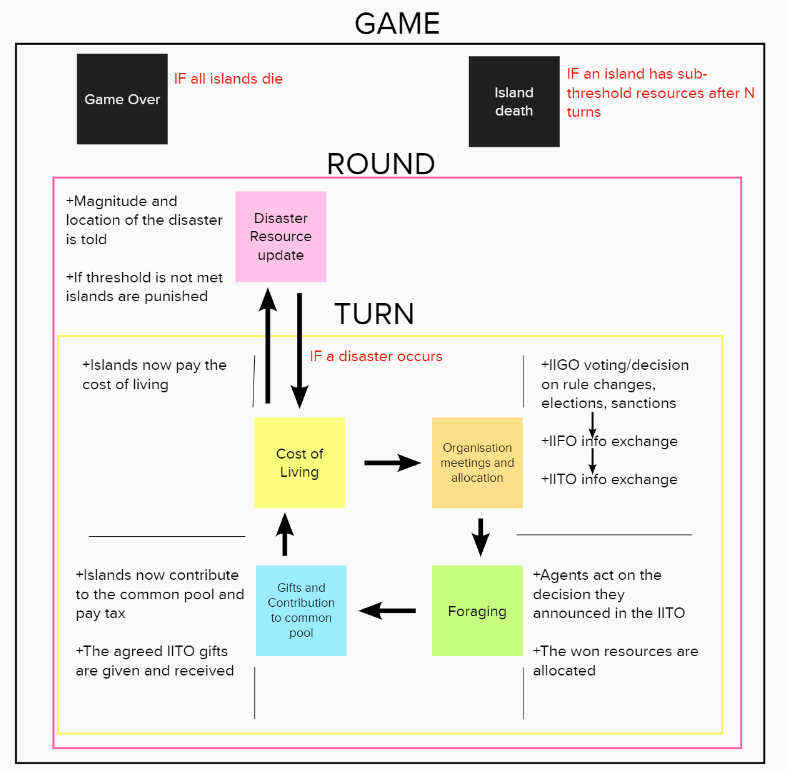
\includegraphics{gamespec-flow.png}
    \caption{High Level Game Specification Flow Diagram}
    \label{fig:gamedesign-flow}
\end{figure}

%update figure
%change when updates occur

\end{document}
